\section{Measuring spiking patterns across the network}

-Mark certain neurons as recording
-This can be done as a boolean flag on the neuron to tell it to keep a time
trace of its potential, or by inserting measurement objects into the simulation.
These measurement objects can take the form of 

\section{Comparing spiking patterns between two networks.}

\subsection{Hamming Distance}
Treating spikes as a binary on-off at a given point in time, it is possible to
calculate the hamming distance between two network spiking patters. 

\subsection{Kulbach-Leibler Divergence}

In order to measure the divergence between two distributions, 

\subsection{Earth Mover's Distance (EMD)}

Also known as the `Wasserstein Distance', Earth Mover's Distance is, simply put,
given two different mounds of earth, the amount of earth that would need to be
moved from one to the other such that both mounds are the same. More formally,
given two distributions in N-dimensional space $P, Q$, the Earth Mover's
Distance is the N-dimensional distance between them. While more computationally
expensive to calculate than Kulbach-Leibler divergence, EMD is symmetric, and
more importantly, is aware of metric space when comparing distributions.

\begin{figure}[ht]
    \begin{subfigure}{.5\textwidth}
        \centering
        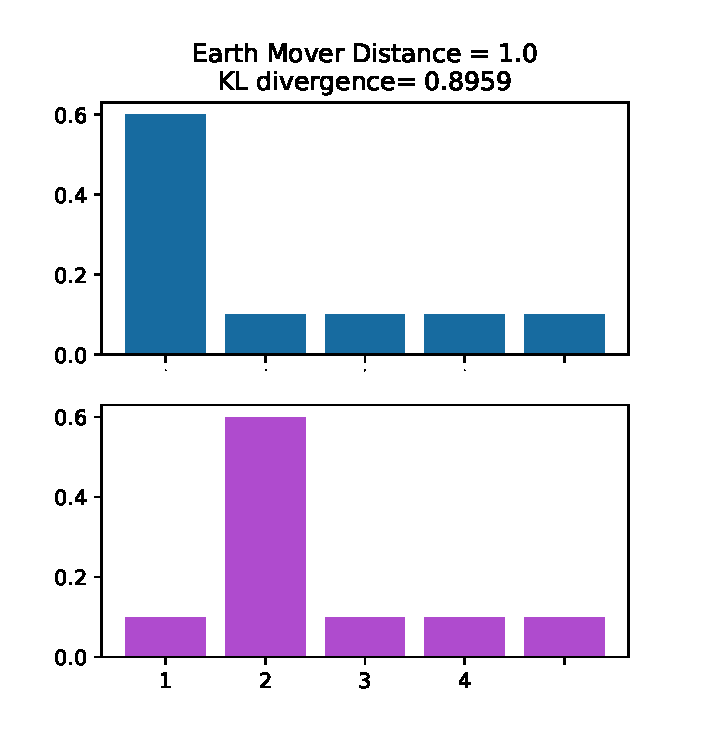
\includegraphics[width=1.0\linewidth]{figures/graphs/EMDvsKLclose.eps}
        \caption{Close distributions have a low EMD}
        \label{fig:LIFSingleSpikeGraph}
    \end{subfigure}%
    \begin{subfigure}{.5\textwidth}
        \centering
        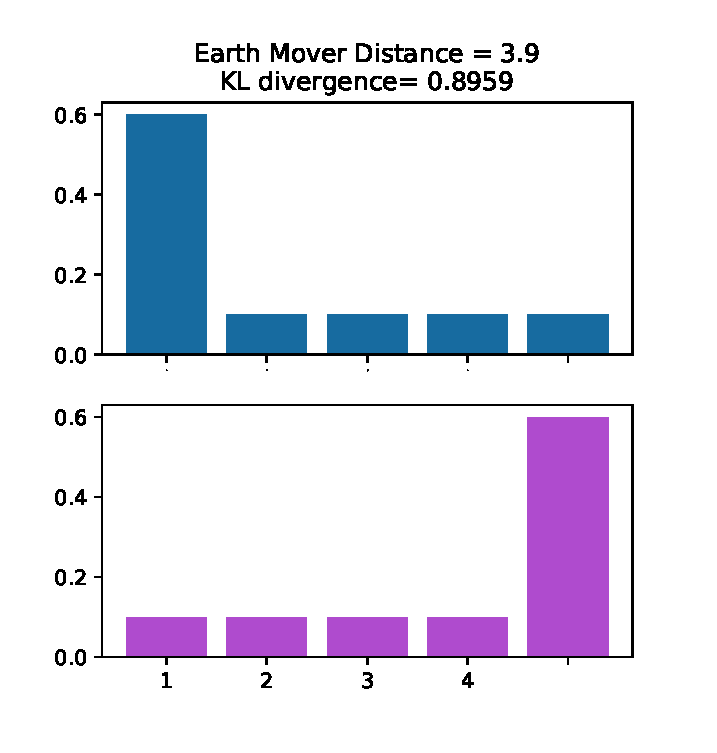
\includegraphics[width=1.0\linewidth]{figures/graphs/EMDvsKLfar.eps}
        \caption{Higher distance between distributions isn't reflected by KL divergence}
        \label{fig:LIFCode}
    \end{subfigure}
    \caption{Comparison between Earth Mover Distance and Kulbach-Leibler Divergence}
    \label{fig:LIFSingleSpikeGraphCode}
\end{figure}

The implementation used in 

\autocite{pele_fast_2009}
